% !TeX program = xelatex
% The PDF is produced with XeTeX. Vector figures are generated by sekiller.py.
\documentclass[10pt,letterpaper,twocolumn]{article}
\usepackage[left=17mm,right=17mm,top=17mm,bottom=18mm,columnsep=6.4mm,footskip=9mm]{geometry}
\usepackage{fontspec,graphicx,booktabs,xcolor,hyperref}
\setmainfont{Liberation Serif}
\setsansfont{Liberation Sans}
\setmonofont{Liberation Mono}[Scale=0.87]
\definecolor{link}{HTML}{225768}
\definecolor{accent}{HTML}{893B39}
\hypersetup{unicode=true,colorlinks=true,urlcolor=link,citecolor=link,linkcolor=link,
  pdftitle={Bimanual Fingertip Manipulation During Humanoid Push Recovery},
  pdfauthor={Ali Özkurt},
  pdfsubject={A simulation study of reactive stepping and simultaneous pen manipulation}}
\setlength{\parindent}{1em}
\setlength{\parskip}{0pt}
\setlength{\abovedisplayskip}{5pt}
\setlength{\belowdisplayskip}{5pt}
\setlength{\textfloatsep}{8pt}
\setlength{\intextsep}{7pt}
\setlength{\tabcolsep}{3pt}
\emergencystretch=1em
\raggedbottom
\makeatletter
\renewcommand\section{\@startsection{section}{1}{0pt}{2.3ex plus .4ex minus .3ex}{.85ex}{\normalfont\fontsize{13}{15}\selectfont\bfseries}}
\renewcommand\subsection{\@startsection{subsection}{2}{0pt}{1.7ex plus .4ex minus .2ex}{.55ex}{\normalfont\fontsize{10.5}{12}\selectfont\bfseries}}
\makeatother
\newcounter{plate}
\newcommand{\figcap}[2]{\refstepcounter{plate}\label{#1}\par\vspace{3pt}\noindent{\fontsize{8.8}{10.6}\selectfont\textbf{Fig. \theplate.}\enspace #2\par}\vspace{4pt}}
\newcommand{\figfile}[1]{\par\smallskip\noindent\includegraphics[width=\linewidth]{sekiller/#1.pdf}\par}
\newcommand{\sidelabel}[1]{{\sffamily\fontsize{8.1}{9.2}\selectfont\bfseries #1}}
\newcommand{\topic}[1]{\par\smallskip\noindent\textbf{#1.}\enspace}
\newcommand{\film}{\href{https://drive.google.com/file/d/1ie0wmTbqMH5YB14TXsx_susyWOL8ietK/view?usp=drivesdk}{Experiment video}}
\newcommand{\code}{\href{https://github.com/ozkurt23/humanoid-dual-pen-recovery}{Project repository}}
\begin{document}
\twocolumn[{
\begin{center}
\vspace*{0.2em}
{\fontsize{23}{26}\selectfont\bfseries Bimanual Fingertip Manipulation During\\ Humanoid Push Recovery\par}
\vspace{.65em}
{\fontsize{14}{17}\selectfont Ali Özkurt\par}
\vspace{.25em}
{\fontsize{9.8}{12}\selectfont November 17, 2026\quad$\cdot$\quad\film\quad$\cdot$\quad\code\par}
\end{center}
\vspace{3pt}
\noindent\begin{minipage}[t]{.327\linewidth}
\sidelabel{(a) Recovery stance}\\[2pt]
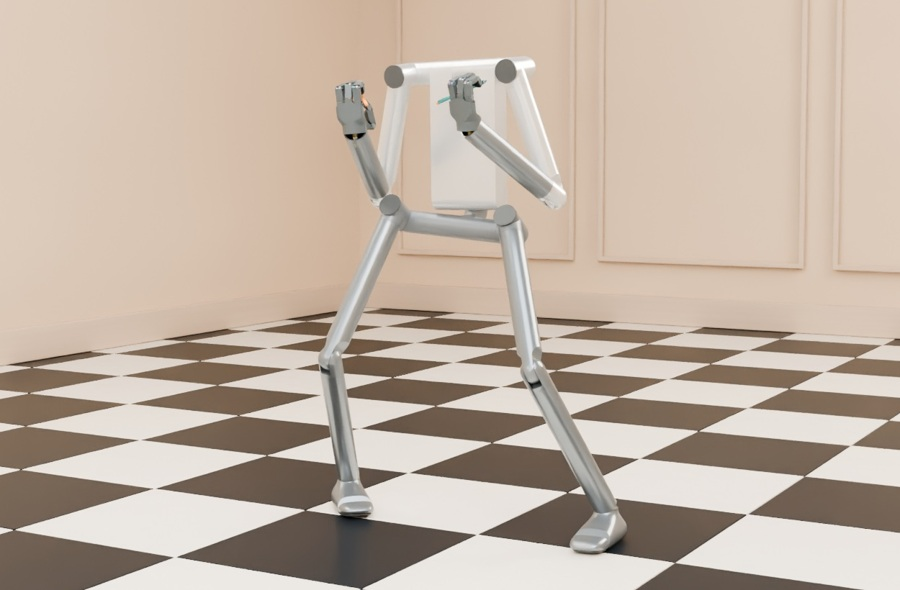
\includegraphics[width=\linewidth]{gorseller/teaser-body.jpg}
\end{minipage}\hfill
\begin{minipage}[t]{.327\linewidth}
\sidelabel{(b) Left fingertip grasp}\\[2pt]
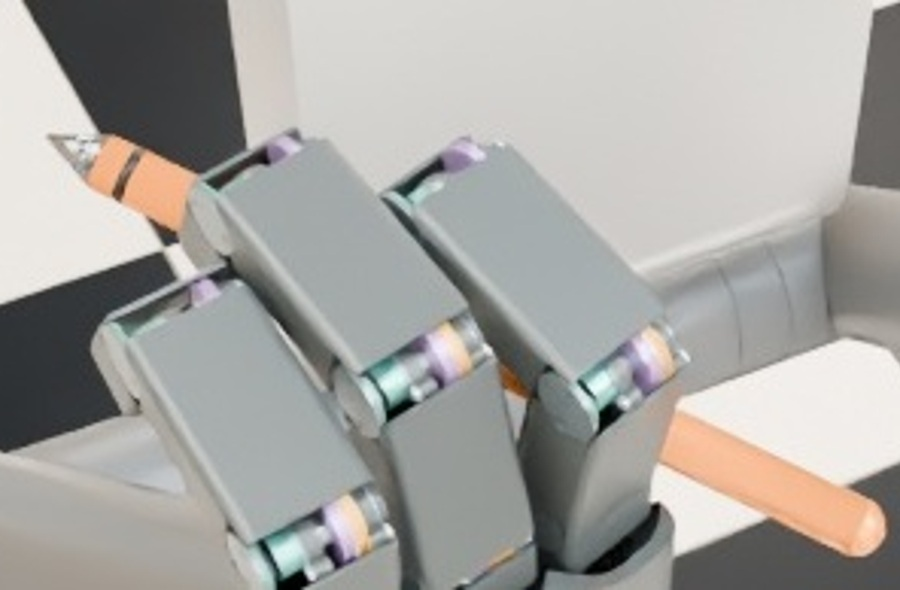
\includegraphics[width=\linewidth]{gorseller/teaser-left.jpg}
\end{minipage}\hfill
\begin{minipage}[t]{.327\linewidth}
\sidelabel{(c) Right fingertip grasp}\\[2pt]
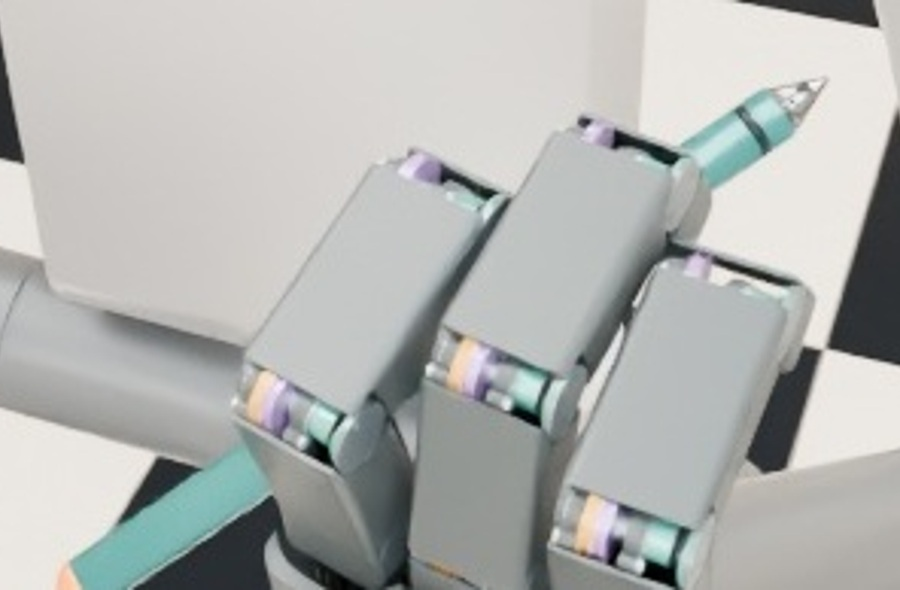
\includegraphics[width=\linewidth]{gorseller/teaser-right.jpg}
\end{minipage}
\figcap{fig:teaser}{Simultaneous views of one physics state at 18.50 s. A lateral push with a 107.7 N plateau acts at the pelvis while the robot manipulates two freely moving pens. The orange pen is in the left hand and the green pen is in the right. The wrist-mounted views resolve finger motion that is difficult to see in the whole-body view.}
\vspace{7pt}
}]
\noindent\textbf{\textit{Abstract}---}
Recovering from a push can displace the hands enough to obscure whether an object is moving within the grasp. We study a simulated humanoid that walks forward while oscillating one pen between the fingertips of each hand. A model-based controller estimates lateral loading from realized dynamics and evaluates candidate foot placements in copies of the current MuJoCo state. Tendon commands continue throughout recovery. Twelve of fifteen runs satisfied a joint criterion requiring five recovery steps, renewed forward progress, and bilateral fingertip manipulation. Five of six schedules reserved after the controller was fixed met the same criterion. In the filmed run, steps in the push direction measured 15.2--29.4 cm and the pen axes reoriented by 28.4--33.9$^\circ$ relative to their respective wrists during individual pushes. Matched rollouts with the force omitted separated the effect of each push from nominal gait. The experiment covers lateral pelvic pushes on one simulated robot.
\section{Introduction}
A robot carrying objects has two obligations during a disturbance. It must create a new support region and keep controlling the objects while the upper body moves. A still image of a pen between fingertips establishes neither continued manipulation nor a successful recovery. This motivates three measurements: foot displacement during an unloaded swing, forward travel after the force vanishes, and object motion expressed in the frame of its own hand.

We combine a walking humanoid and two tendon-driven V3 hands in one articulated simulation. A disturbance generator chooses five lateral pushes. Its schedule is hidden from the controller. We test whether the robot can step toward the push and resume walking while preserving both grasps. Matched replays omit each push in turn to separate its effect from nominal gait.
\topic{Contributions}
We combine causal foot-placement search with wrist-relative manipulation scoring. Two matched interventions isolate the effects of external force and of a return-to-gait rule.
\section{Related Work}
Eureka uses language-model-generated reward code and reinforcement learning to produce dexterous pen-spinning behaviors in a simulated Shadow Hand~\cite{eureka}. It motivates our choice of object and skill. Our experiment uses a periodic tendon command and grades relative pen reorientation during recovery. The measured motion is oscillatory.

Capture-point analysis relates recovery stepping to the state of a disturbed biped~\cite{capture}. We evaluate foot placements by advancing the articulated contact model in MuJoCo~\cite{mujoco}. Recent learned systems address other forms of generalization: $\pi_{0.5}$ combines heterogeneous training data to perform manipulation in unfamiliar environments~\cite{pi}, and DreamZero jointly predicts future video and actions for robot control~\cite{dream}. Here the model is explicit and the evaluated variation is the load schedule. We evaluate perturbation-response generalization within this model and explicitly account for incomplete exposures.
\topic{Study questions}
Does the fixed controller succeed outside the original five-push sequence? Do the pen and foot measurements show genuine relative motion? How much does the response change when the external force or the stance-closing rule is removed?

\clearpage
\section{System and Control}
\subsection{Mechanical model}
A floating-base humanoid carries mirrored V3 tendon hands. Each hand holds a separate free pen. Finger contact transmits normal and tangential forces in the simulation. A joint-space inverse-dynamics tracker and contact-constrained ankle wrench allocation produce the whole-body commands. MuJoCo advances the full state every 2 ms. Hand and body poses are sampled at 60 Hz for independent measurement and rendering.
\subsection{Sensing a surprise push}
At every step, the observer estimates the applied lateral load from the previous simulated acceleration, inertial terms, and realized contact reactions. In the lateral floating-base row, the residual has the form
\begin{equation}
  \widehat F_x=\big[M(q)\ddot q+h(q,\dot q)-f_{\rm passive}-f_{\rm constraint}\big]_x .
\end{equation}
Here $M$ is the joint-space mass matrix, $h$ the bias force, and the last two terms are passive and constraint forces. The controller has access to simulated dynamics quantities; estimating equivalent signals on hardware is a separate problem. The external load generator does not supply its next onset, force direction, or release time to the controller.
\figfile{controller}
\figcap{fig:system}{The load schedule acts on the main physics state. The controller forecasts from the realized dynamics residual and updates tendon amplitude from wrist-relative pen pose.}
\subsection{Choosing a recovery step}
When the absolute lateral residual reaches 2 N outside an active recovery, the controller creates independent forward simulations initialized from the current state. Candidate responses vary the swing leg, landing position, timing, and ankle support. An initial screening evaluates 20 candidates. For a promising candidate, the search checks profiles with assumed plateau durations of 1.0, 1.5, and 2.0 s. If its predicted cost is high, or if support is wide, the search considers additional responses. Difficult cases trigger a further set of short, low steps. The physical rollout receives only the selected control.
\topic{Returning to walking}
A wide fore--aft stagger can leave the scheduled swing foot already far ahead of its partner. Taking another forward stride then preserves a poor starting stance for the next push. When this geometry is detected, the first swing narrows the lateral separation before forward stepping resumes. For development schedule 714, stance width before the fifth push fell from 0.79 to 0.49 m after this change. This is a diagnostic observation for one schedule.
\newpage
\subsection{Bilateral fingertip control}
The two hands receive periodic tendon commands with a 3.2 s cycle. A 60 Hz monitor compares the pen center in wrist coordinates with its starting position. An inward displacement toward the palm greater than 6.8 mm, or an increase in the absolute longitudinal coordinate greater than 10 mm, triggers a smooth reduction to 75\% amplitude in the affected hand. The other hand continues its own motion. The monitor has access to simulator object pose.
\begin{center}\setlength{\tabcolsep}{1.4pt}\sffamily\fontsize{7.6}{9}\selectfont
\begin{tabular}{@{}rccc@{}}
 & 17.48 s & 18.50 s & 20.15 s \\
 L &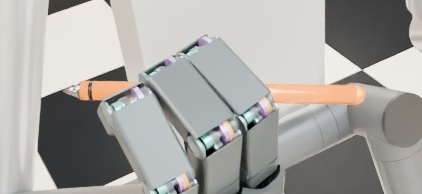
\includegraphics[width=.285\linewidth]{gorseller/L-1050.jpg}&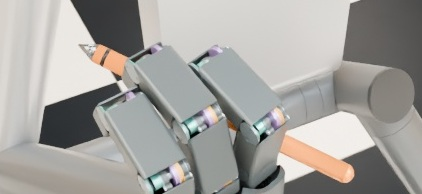
\includegraphics[width=.285\linewidth]{gorseller/L-1111.jpg}&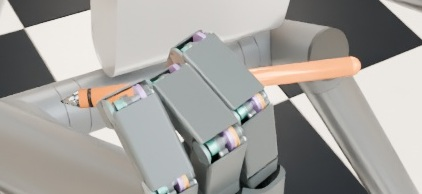
\includegraphics[width=.285\linewidth]{gorseller/L-1210.jpg}\\
 R &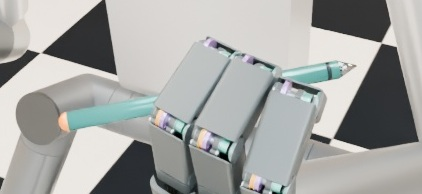
\includegraphics[width=.285\linewidth]{gorseller/R-1050.jpg}&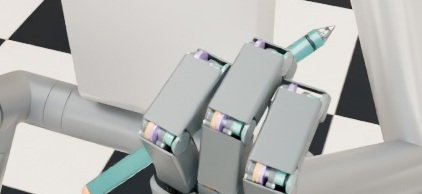
\includegraphics[width=.285\linewidth]{gorseller/R-1111.jpg}&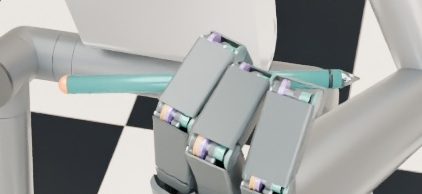
\includegraphics[width=.285\linewidth]{gorseller/R-1210.jpg}
\end{tabular}\end{center}
\figcap{fig:hands}{Wrist-fixed image sequences during the second push. Columns show synchronized samples; rows show opposite hands.}
\section{Experimental Protocol}
\subsection{Disturbance schedules}
Each trial lasts at most 55 s and contains five scheduled pelvic pushes along the lateral axis. Four earlier schedules preserve the sequence of peak magnitudes 60, 75, 85, 100, and 115 N and vary event timing and initial sign. In the other eleven schedules, event $j$ begins within a window $[3,7.5]+10.3j$ s, $j=0,\ldots,4$. Peak magnitude is sampled from 60--115 N, plateau duration from 1--2 s, and ramp duration from 0.85--1.35 s. Rise and fall share a duration within each event, and direction is sampled for each push.
\subsection{Pass criteria}
A trial must complete 55 s without non-foot ground contact. At every push a foot must be unloaded for at least 30 ms, rise at least 5 mm, and land at least 3 cm along the force direction. The pelvis must move at least 2 cm forward from full release to the next onset or recording end. Both pens must have opposed fingertip contact in at least 98\% of the trial samples and zero palm contact. In each push window each pen axis must sweep at least 15$^\circ$ in its own wrist frame.

\topic{Experimental controls}
We reserve six schedules after the controller is fixed, retain early stops, and report both event and trial denominators. A force-omission comparison tests whether the external load changes the motion. A separate single-factor ablation disables the lateral-first stance-closing rule while preserving the prescribed loads, model, and remaining controller settings. These interventions answer different questions.
\clearpage
\section{Experimental implementation and rendering pipeline}
\subsection{From source geometry to a runnable model}
The experiment was built on a single Ubuntu workstation. The source CAD is the project's private \texttt{priv\_humanoid} repository at revision \texttt{171930c}. A Python assembly script loads the humanoid MJCF and repaired V3 hand model, computes a forward-facing arm pose, and replaces the original hand assemblies at the wrist joints. The two hands receive separate joint and tendon names and one pen each. Each pen has a free joint. The combined MJCF uses gravity of 9.81 m/s$^2$, the implicit-fast integrator, an elliptic friction cone, and the Newton solver with a limit of 30 iterations per 2 ms step.

\subsection{From a schedule to a trajectory}
The Python experiment runner selects a disturbance schedule by seed, constructs its time-varying loads, and advances the coupled model in MuJoCo 3.8.0. Candidate foot placements run in additional CPU processes on the same Intel Core Ultra 9 275HX. The local model copies are disposable: only the selected action is applied to the continuing physical trajectory. This preserves one continuous history for walking, finger contacts and pen motion. Wall-clock planning time is distinct from simulated time.

For each run the physics loop writes time, applied lateral force, pelvis state, foot contacts and grasp diagnostics at 500 Hz. A separate 60 Hz trace stores joint positions and named body poses for reconstruction. The evaluator uses force onsets and releases to extract event windows; it scores landings from contact and ankle position, walking from pelvis displacement, and pen reorientation from wrist and pen orientations. The complete set of seeds is reported with its failed cases in Table~\ref{tab:trials}.

\begin{center}
\sidelabel{(a) Recorded joint state in MuJoCo}\\[2pt]
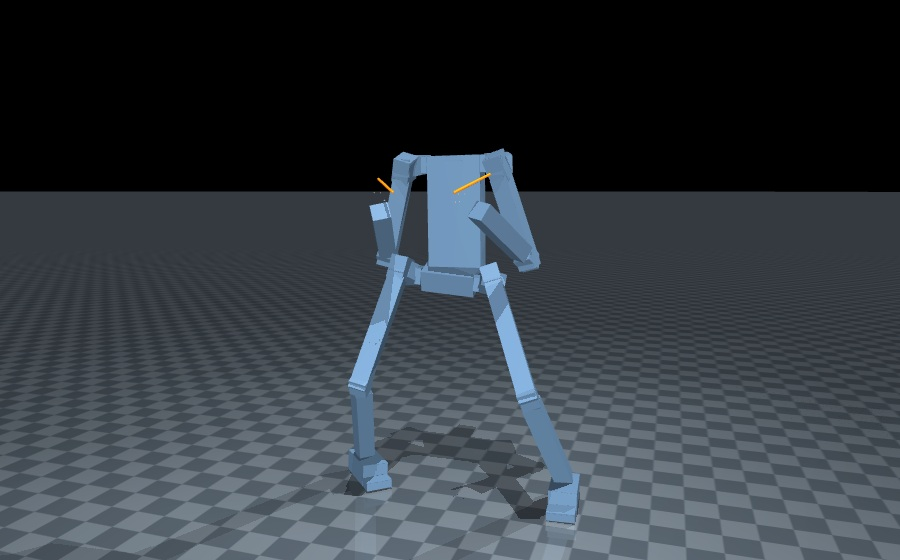
\includegraphics[width=.9\linewidth]{gorseller/physics-state.jpg}
\end{center}
\figcap{fig:physics}{The stored joint state at 18.50 s loaded back into MuJoCo. This view shows the articulated simulation geometry. Gravity, contacts and the applied load were resolved during the original rollout.}
\newpage
\subsection{From trajectory to film}
The Blender 4.5.16 production scripts bind the recorded positions and quaternions to named robot links, including the two V3 hand assemblies. The same pose samples place the pen bodies in each shot. Quaternion signs are made continuous before animation curves are written. A level studio floor, soft lights and contrasting pens aid inspection of contact and foot placement.

The full take has 3,301 pose samples including the endpoint. The first 3,300 samples drive the 55 s film at 60 frames/s. Ten cameras show the same recording in consecutive 5.5 s shots. During two push intervals, wrist-locked close-ups reuse the same frame numbers as the body view. Cycles renders the images on the workstation's NVIDIA GeForce RTX 5090 Laptop GPU with OptiX acceleration and denoising.

\begin{center}
\sidelabel{(b) Blender scene before overlays}\\[2pt]
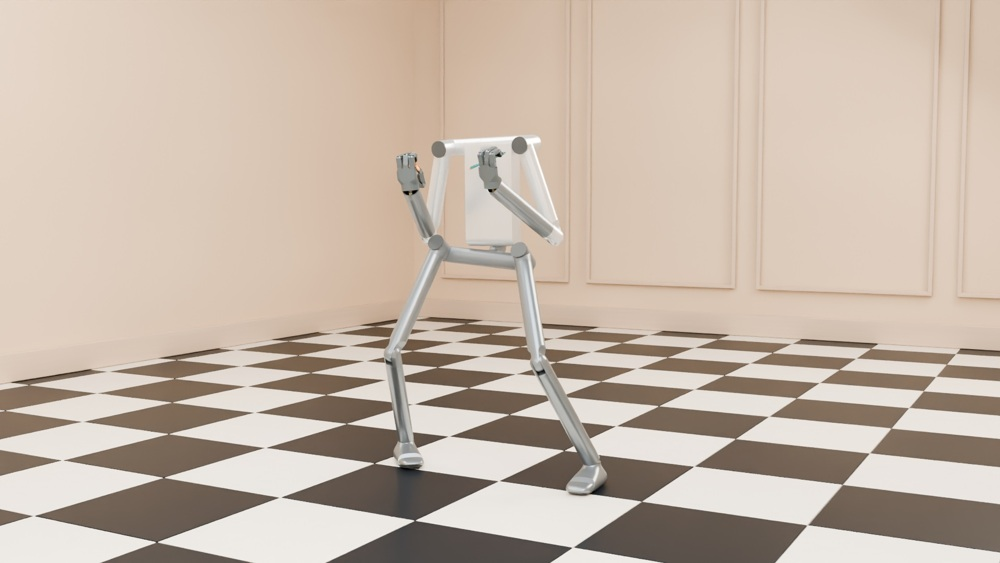
\includegraphics[width=.95\linewidth]{gorseller/blender-state.jpg}\\[4pt]
\sidelabel{(c) Decoded H.264 frame}\\[2pt]
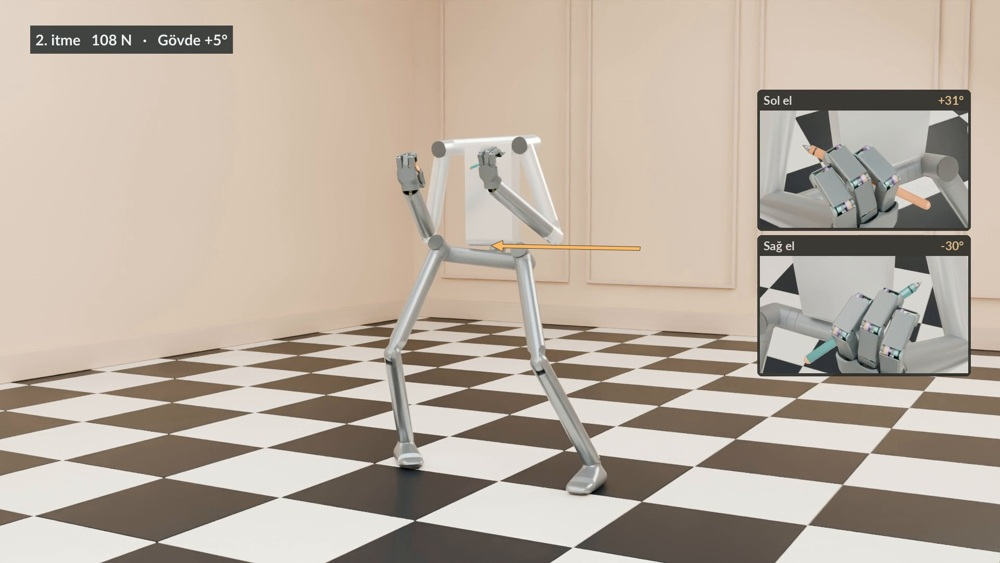
\includegraphics[width=.95\linewidth]{gorseller/encoded-frame.jpg}
\end{center}
\figcap{fig:encoding}{The same instant as Fig.~\ref{fig:physics}, before and after compositing. The encoded view adds the load direction, captions, and synchronized left and right wrist views.}
\subsection{Encoding and verification}
Python assembles the force and object-angle captions, wrist-inset overlays and chapter metadata, then invokes FFmpeg to encode H.264 at 1,920 by 1,080 pixels. The encoder uses a constant rate factor of 16. The finishing script reopens the output, checks frame count, duration, frame rate and image dimensions, and decodes frames from nine points in the film to check image content. The underlying pose and force logs remain available independently of the encoded video.

\clearpage
\section{Results}
\subsection{Trial-level evaluation}
We evaluated 15 schedules with the same final controller. The earlier comparison group passed four of four, the film and additional development cases passed three of five, and the six schedules reserved after fixing the controller passed five of six. Table~\ref{tab:trials} retains incomplete trials in the denominator.
\begin{center}
\refstepcounter{table}\label{tab:trials}
{\fontsize{8.7}{10.5}\selectfont\textbf{Table \thetable.} Per-schedule outcomes. Step and walk counts use five scheduled events. The last six rows form the reserved evaluation.\par}
\vspace{3pt}
\fontsize{8.1}{10}\selectfont\setlength{\tabcolsep}{2.4pt}\renewcommand\arraystretch{1.08}
\begin{tabular*}{\linewidth}{@{\extracolsep{\fill}}lrrrrcc@{}}\toprule
ID & Time (s) & Path$^*$ (m) & Steps & Walk & Palm & Result\\ \midrule
714 & 55.000 & 2.00 & 5/5 & 5/5 & No & Pass \\
715 & 55.000 & 1.97 & 5/5 & 5/5 & No & Pass \\
716 & 55.000 & 1.92 & 5/5 & 5/5 & No & Pass \\
727 & 55.000 & 1.97 & 5/5 & 5/5 & No & Pass \\
905 & 55.000 & 1.97 & 5/5 & 5/5 & No & Pass \\
924 & 55.000 & 1.94 & 5/5 & 5/5 & No & Pass \\
\textcolor{accent}{\bfseries 1042} & 17.518 & 0.60 & 1/5 & 1/5 & Yes & Fail \\
1051 & 55.000 & 2.18 & 5/5 & 5/5 & No & Pass \\
\textcolor{accent}{\bfseries 1052} & 25.970 & 0.94 & 3/5 & 2/5 & No & Fail \\
\textcolor{accent}{\bfseries 1071} & 48.682 & 1.10 & 5/5 & 4/5 & Yes & Fail \\
1072 & 55.000 & 1.93 & 5/5 & 5/5 & No & Pass \\
1073 & 55.000 & 1.80 & 5/5 & 5/5 & No & Pass \\
1074 & 55.000 & 1.94 & 5/5 & 5/5 & No & Pass \\
1075 & 55.000 & 1.79 & 5/5 & 5/5 & No & Pass \\
1076 & 55.000 & 1.99 & 5/5 & 5/5 & No & Pass \\
\bottomrule
\end{tabular*}
{\fontsize{8}{9}\selectfont $^*$Net forward pelvis displacement from the initial position.\par}
\end{center}
\topic{Failure modes}
Trial 1042 stopped at 17.52 s after two same-direction pushes near 109 N. It failed the second recovery and recorded palm contact. Trial 1052 stopped at 25.97 s. It had three qualifying lateral steps but only two subsequent walking intervals. The reserved failure, trial 1071, stopped at 48.68 s. Its fifth lateral step qualified and palm contact occurred. The load was still active when tracking stopped, so post-release walking could not be measured. Thus a count of lateral steps alone would have missed this failure. The rollout stops when horizontal tracking error exceeds 0.65 m on either axis, or vertical error exceeds 0.30 m. The first two runs exceeded the vertical threshold, and 1071 exceeded the fore--aft threshold. No non-foot ground contact was logged before these stops.
\subsection{Exposure and onset phase}
Across 75 planned pushes, 70 began and 67 reached full release. All 67 complete exposures had a qualifying landing and subsequent forward progress. In 62 of those events a qualifying swing began after onset. In the other five the foot was already airborne. A post-onset lift establishes the order of events. Swing timing also depends on gait phase. Appendix~\ref{sec:event-audit} reports the support-state strata and hand contact distributions.
\newpage
\subsection{A continuous filmed trial}
Trial 924 reached 1.94 m net forward travel. Each of its five recoveries included a foot lift and landing toward the force, followed by forward travel. Figure~\ref{fig:force} gives the timing against pelvis position, and Fig.~\ref{fig:steps} reports the two displacements separately.
\figfile{yuk-ve-yuruyus}
\figcap{fig:force}{Applied lateral force and cumulative forward pelvis displacement in trial 924. Shading covers periods of applied load.}
\figfile{adimlar}
\figcap{fig:steps}{Longest qualifying lateral landing at each push and net forward pelvis travel after release. Travel ends at the next push onset or at the end of the run.}
The second push began at 17.22 s and held a 107.7 N peak for 1.82 s. The foot landed 29.4 cm along the push direction. After release, the pelvis moved 30.2 cm forward before the third push. Across all five recoveries, the first subsequent swing that landed at least 3.5 cm forward began 2.16--2.25 s after full release.

\clearpage
\subsection{Pen motion relative to the wrist}
Let $u_h(t)$ be the unit pen axis in wrist $h$’s frame. For a push window $I$ we measure
\begin{equation}
\theta_h(I)=\max_{s,t\in I}\arccos\big(u_h(s)^{\mathsf T}u_h(t)\big).
\end{equation}
The two wrists can rotate without changing this quantity. In trial 924 the peak pairwise angular change was 28.4--33.9$^\circ$ across all ten hand--event pairs. At the second push, both hands reached 33.9$^\circ$. Opposed fingertip contact occupied 99.95\% of physics samples on the left and 99.78\% on the right. Neither pen touched a palm.
\figfile{kalemler}
\figcap{fig:angles}{Signed inclination of the pen axis projected into each wrist's $x$--$z$ plane. Shading marks the second push. The three-dimensional criterion in Eq.~(2) uses the full three-dimensional axis.}
\begin{center}
\refstepcounter{table}\label{tab:windows}
{\fontsize{8.7}{10.4}\selectfont\textbf{Table \thetable.} Filmed load windows and maximum wrist-relative angular excursions. Signs denote lateral load direction.\par}
\vspace{3pt}
\fontsize{8.8}{10.5}\selectfont
\begin{tabular*}{\linewidth}{@{\extracolsep{\fill}}crrrrr@{}}\toprule
Push & Onset (s) & Peak (N) & Hold (s) & Left ($^\circ$) & Right ($^\circ$)\\\midrule
1 & 6.10 & $-$62.8 & 1.77 & 32.8 & 33.6\\
2 & 17.22 & $-$107.7 & 1.82 & 33.9 & 33.9\\
3 & 27.04 & 103.6 & 1.30 & 30.6 & 28.4\\
4 & 34.88 & 104.8 & 1.23 & 30.9 & 30.5\\
5 & 45.96 & $-$63.2 & 1.70 & 32.3 & 33.9\\\bottomrule
\end{tabular*}\end{center}
\topic{Contact interpretation}
Opposed contact requires a thumb pad and a pad on another digit to touch the pen simultaneously. The primary fraction is evaluated over all physics samples in each recorded run. Per-push reorientation is an additional condition. One high time-averaged contact value alone therefore cannot certify that a pen kept moving during every disturbance.
\newpage
\subsection{Force-omission controls}
We replayed the same pre-event choices and removed one push at a time in five paired simulations. For each pair, the 500 Hz movement measurements matched exactly before onset. We then subtracted lateral pelvis position in the omitted-force run from that in the original, taking the push direction as positive.
\figfile{eslenmis}
\figcap{fig:paired}{Signed original-minus-control pelvis displacement in cm. The first two columns use elapsed time after onset; the last two use points on each applied load profile.}
\figfile{matched-traces}
\figcap{fig:traces}{Continuous matched differences through release, with every push aligned to its own onset. Dots mark release. The durations differ because the pulse profiles were sampled separately.}
The first response initially opposed the push: after 1 s the pelvis was 6.2 cm farther in the opposite direction than in the no-push control. By the end of the force plateau, the difference was positive for all five events, from 4.2 to 40.0 cm. It remained positive after load removal. The early countermotion and later yielding are both visible in the comparisons.
\topic{Interpreting the film}
A forward-facing view can hide relative pen motion while making an early counter-movement look like steady bracing. The wrist-frame angles and the matched trajectories resolve these two ambiguities separately. The signed differences are specific to the recorded robot state at each onset. They do not establish the response one would obtain after a different sequence of preceding pushes.
\twocolumn[{
\section{Ablation of the return-to-gait rule}
\centerline{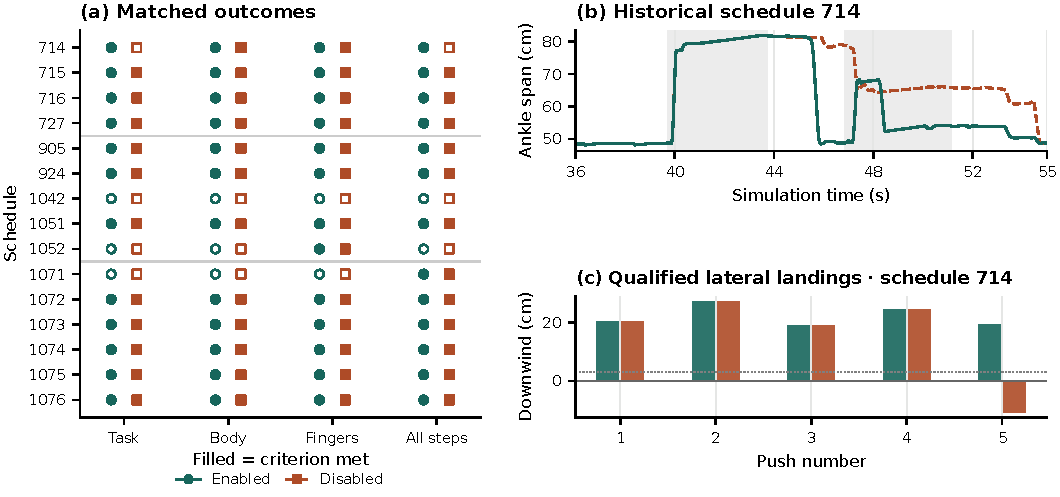
\includegraphics[width=.94\linewidth]{sekiller/ablation.pdf}}
\figcap{fig:ablation}{Paired trials with lateral-first stance closure enabled or disabled. (a) Filled markers indicate a passed criterion. (b) Ankle span in the historical example, with shading for load exposure. (c) Largest signed landing of an unloaded foot per push in the same trial. The dotted line is the 3 cm criterion.}
\vspace{5pt}
}]
\noindent We reran each schedule with a single change: the Boolean gate for a lateral-first restart was forced off in both the candidate rollouts and the live controller. The default gate requires an ankle span greater than 1.5 times nominal stance width, a fore--aft stagger above 5.5 cm, and a different scheduled swing foot from the one chosen to close the stance. Ordinary lateral recovery and the remaining width correction operate in both arms. Applied-force samples matched exactly over each pair's common recorded interval.
\topic{Matched outcomes}
Both variants passed eleven schedules and failed three. One historical case passed only with the gate enabled. Aggregate joint success thus changed from 11/15 with the gate disabled to 12/15 with it enabled. Eleven pairs produced identical complete trace arrays. Among the six reserved schedules both variants passed five. These results locate a specific failure that the rule corrects; the paired evaluation observed no increase in reserved-schedule success.
\topic{Historical schedule 714}
The 500 Hz measurements first differed at 44.406 s. At the onset of the fifth push, stance width was 48.7 cm with the rule enabled and 78.9 cm without it. The largest signed lateral landing in that window changed from 10.7 cm opposite the push to 19.2 cm along it. Both variants stayed upright for 55 s, resumed forward motion after every load, and covered 1.999 m overall. The joint outcome changed because of landing direction.

\section{Discussion}
The experiment uses one robot, one pair of hands, one level floor and two lateral force directions at the pelvis. The six reserved schedules give a small test of timing and load variation. Fore--aft disturbances, other contact locations, changed friction and sensor noise remain untested. Parallel forward simulation may take longer than the corresponding simulated interval. Hardware transfer and real-time execution have not been measured. The hand objective concerns a bounded reorientation; continuous full revolutions were outside this experiment.
\section{Conclusion}
Twelve of fifteen simulated runs completed concurrent recovery stepping, forward walking, and two-pen manipulation. On the six reserved schedules the controller completed five. Checking wrist-relative motion alongside recontact and walking exposed failures that any one measure would conceal. The stance-closing ablation improved one historical landing and left reserved-schedule success unchanged.
\begin{thebibliography}{9}\fontsize{8.6}{10.2}\selectfont\raggedright
\bibitem{eureka} Y. J. Ma et al. \href{https://eureka-research.github.io/}{Eureka: Human-Level Reward Design via Coding Large Language Models}. ICLR, 2024.
\bibitem{capture} J. Pratt, J. Carff, S. Drakunov, and A. Goswami. \href{https://doi.org/10.1109/ICHR.2006.321385}{Capture Point: A Step toward Humanoid Push Recovery}. IEEE-RAS Humanoids, 2006.
\bibitem{mujoco} E. Todorov, T. Erez, and Y. Tassa. \href{https://homes.cs.washington.edu/~todorov/papers/TodorovIROS12.pdf}{MuJoCo: A Physics Engine for Model-Based Control}. IEEE/RSJ IROS, 2012.
\bibitem{pi} Physical Intelligence. \href{https://www.physicalintelligence.company/download/pi05.pdf}{$\pi_{0.5}$: a Vision-Language-Action Model with Open-World Generalization}. arXiv:2504.16054, 2025.
\bibitem{dream} S. Ye et al. \href{https://dreamzero0.github.io/DreamZero.pdf}{World Action Models are Zero-shot Policies}. Technical report, NVIDIA, 2026.
\end{thebibliography}
\clearpage
\appendix
% Editable supplement. Requires booktabs. Supports a two-column paper.
\section{Event-level audit}
\label{sec:event-audit}
Each of the 15 frozen-controller schedules specified five lateral loads. Of 75 planned loads, 70 reached onset and 67 reached release. Three runs stopped while a force was active, leaving five later loads unobserved. All event counts below condition on exposure. The primary endpoint remains the joint, 55~s run-level outcome.

\begin{center}\refstepcounter{table}\label{tab:exposure}
\centering
\small
{\fontsize{8.7}{10.4}\selectfont\textbf{Table \thetable.} Observed load onsets by foot support and force sign. A landing may complete a swing already under way. A new swing additionally requires lift-off at or after onset. Release counts complete load windows. The sign rows partition the same 70 events as the support rows.}
\par\vspace{3pt}\fontsize{8.4}{10.2}\selectfont
\begin{tabular}{@{}lrrrr@{}}
\toprule
Onset state & Starts & Landings & New swings & Releases\\
\midrule
Both feet & 42 & 41 & 41 & 41\\
Left only & 12 & 12 & 10 & 12\\
Right only & 16 & 16 & 13 & 14\\
\midrule
Positive world $x$ & 32 & 31 & 29 & 30\\
Negative world $x$ & 38 & 38 & 35 & 37\\
\midrule
All observed & 70 & 69 & 64 & 67\\
\bottomrule
\end{tabular}
\end{center}

\topic{Landing versus initiating a step}
A qualifying landing shifts at least 3~cm along the force direction after at least 30~ms without ground contact and at least 5~mm of vertical excursion. All 67 complete loads had a qualifying landing. For 62 of them, a qualifying swing also began after load onset. In the other five the qualifying foot was already airborne. The median maximum signed landing distance per complete load was 19.2~cm (range 7.5--30.6). Subsequent forward travel, measured from release to the next load or the end of the run, had a median of 34.7~cm (3.1--60.4). The individual windows span different durations.

\topic{Object motion and contact}
During the 67 complete loads, the median maximum shaft-axis excursion relative to the wrist was $31.4^\circ$ on the left and $32.3^\circ$ on the right. No palm contact occurred within these 67 windows. For 66 windows, each pen had opposing fingertip contact in at least 98\% of load-window samples. The exception was load~5 of seed~1075, with 97.96\% left-hand contact during the load. The primary run-level criterion uses contact aggregated over the full recording; this seed passed at that scale.

\topic{Where evaluation stopped}
Seed~1042 stopped on its second load at 17.518~s, and seed~1052 stopped on its third at 25.970~s. Each crossed the 0.30~m vertical tracking-error limit. Seed~1071 stopped on its fifth load at 48.682~s, crossing the 0.65~m horizontal tracking-error limit along the fore--aft axis. At each stop the force was still active. A post-release walking distance therefore cannot be measured for those three events. The recorded run-level palm contacts occurred in 1042 and 1071.

\topic{Sampling uncertainty}
Five of six newly reserved schedules passed. Under an independent, equal-probability Bernoulli model for schedules from the same generator, the two-sided 95\% exact binomial interval is 35.9--99.6\%. The small denominator limits precision. Events within a run share robot state and are unsuitable as independent replicates of full-task success. All tests used one simulated robot, terrain and lateral force application site.


\section{Reproduction details}
\subsection{Local planning objective}
The observer uses 500 Hz simulator dynamics. A history of up to 100 residual samples informs the candidate force forecast. The short-horizon instability score at simulation step $k$ is
\begin{equation}
J_k=5|e_x|+8|e_y|+15\max(0,z_0-z_k-0.14)+0.12\|\omega_{1:2}\|.
\end{equation}
Here $e_x,e_y$ are horizontal root tracking errors, $z_0-z_k$ is height loss in metres, and $\omega_{1:2}$ is the logged two-axis angular-velocity component. A predicted score exceeding 4 or an excessive mount-to-pen distance terminates a candidate with a penalty. Otherwise the cost combines the worst and integrated instability, missed opposed contacts, terminal speed and signed displacement along the push. This evaluated cost is separate from the external task-success rubric used in Table~\ref{tab:trials}.
\subsection{Simulation, analysis, and rendering}
Restore the archive from the \code, install the listed simulation dependencies, and run \texttt{bash work/parmak\_denge/run.sh 924} to reproduce the filmed run. The 60 Hz poses and 500 Hz physics traces are recorded before rendering.

\topic{Coordinate conventions}
The lateral direction is world $x$, with the positive direction chosen separately for each signed landing and each force-omission difference. Forward displacement is the signed change in the pelvis coordinate along the walking axis. Pelvis travel and foot placement measure different bodies, directions and intervals. The first force-onset time in the film uses the first nonzero sample; the event audit starts at $|F|>0.002$ N. Their timestamps can differ by a few milliseconds.

\topic{Clocks and sample counts}
A 55 s run includes 3,301 pose samples at 60 Hz when the initial and final states are both counted. The accompanying film uses 3,300 frames at 1,920 by 1,080 pixels and 60 frames/s. Contact and force traces use the 500 Hz physics clock. Discrete pose frames bracket foot lift and landing; the implemented thresholds apply to those samples.

\topic{Files used for this paper}
The source directory includes plots, numerical tables, crop provenance, and regeneration scripts. Incomplete outcomes remain missing in the event audit. Trial 924 is included in Table~\ref{tab:trials}.


\end{document}
